\chapter{Evaluation}\label{ch:evaluation}
Das folgende Kapitel dient dem Vergleich zwischen der entwickelten Datenstruktur und der bisherigen Organisation der Bloom-Filter in AMBIENCE. Abschnitt \ref{sec:datensatz} beschreibt zunächst den für die Evaluation verwendeten Datensatz. Dieser stammt nicht aus AMBIENCE, sondern die Bloom-Filter wurden wie in Abschnitt \ref{sec:umsetzung} beschrieben selbst implementiert. Der Versuchsaufbau, d.h. welche Aspekte der Indexstruktur untersucht und verglichen wurden, findet sich in Abschnitt \ref{sec:versuchsaufbau}. Die erzielten Ergebnisse werden in Abschnitt \ref{sec:ergebnisse} vorgestellt und in Abschnitt \ref{sec:interpretation} ausgewertet. 
\section{Datensatz}\label{sec:datensatz}
Obgleich nicht mit echten AMBIENCE-Daten gearbeitet wurde, wurde ein möglichst realistisches Szenario erstellt mit folgenden Parametern:
\begin{center}
\begin{table}[htbp]
{\small
\begin{center}
\begin{tabular}[center]{lcc}
\toprule
\textbf{Filtergröße} & 256 Bit & 512 Bit\\
\midrule
\textbf{Anzahl Bloom-Filter (m)} & 100 & 100\\
\midrule
\textbf{Anzahl eingefügte Objekte (n)} & 50 & 50\\
\midrule
\textbf{Anzahl Hashfunktionen (d)} & 4 & 8\\
\bottomrule
\end{tabular}
\end{center}
} % end of tiny
\caption[Datensatz für den Versuchsaufbau]{Datensatz für den Versuchsaufbau.\label{tab:Datensatz}}
\end{table}
\end{center}
Als Wörterbuch wurde die Unix-Datei \texttt{words} verwendet, aus der jeweils 50 zufällige Einträge in die Bloom-Filter eingefügt wurden. Wie in Abschnitt \ref{sec:hashfunktionen} erläutert, wurden zum Einfügen Murmur-Hashfunktionen verwendet. Die Anzahl der zu verwendenden Hashfunktionen lässt sich berechnen als 
% \[d = \lceil\frac{m}{n} * ln(2)\rceil.\]
\[d = \Ceil[\Bigg]{\frac{m}{n} * ln(2)}.\]
\noindent
Der \textit{i+1}-te Hashwert wurde dabei jeweils aus dem \textit{i}-ten Hashwert berechnet wie in Abschnitt \ref{sec:bloom-implementierung} beschrieben. Den Bloom-Filtern wurden zunächst zufällige IDs zugewiesen. Sie wurden jeweils sowohl in einen BloomFilterTree mit 256 bzw. 512 Bit Filtergröße als auch in einen Bloom-Filter-Vektor\footnote{Objekte vom Typ \texttt{std::vector<BloomFilter>}.} eingefügt, der die unsortierte Liste repräsentiert.
\section{Versuchsaufbau}\label{sec:versuchsaufbau}
Der Versuchsaufbau vergleicht die Indexstruktur BloomFilterTree mit einer unsortierten Liste von Bloom-Filtern, was der bisherigen Implementierung in AMBIENCE entspricht. Dazu wurden den Bloom-Filtern zunächst zufällige IDs zugewiesen. Für beide Filtergrößen wurden fünf Experimente durchgeführt:  
\begin{enumerate}
	\item Ergebnisqualität
	\item CPU-Zeit 
	\item Speicherbedarf 
	\item Komplexität 
	\item Aufbaukosten 
\end{enumerate}
\subsection{Ergebnisqualität}\label{sec:ergebnisqualität}
Zur Ermittlung der Ergebnisqualität wurde eine nächste-Nachbarn-Suche und eine 3-nächste-Nachbarn-Suche auf dem BloomFilterTree durchgeführt. Die erzielten Ergebnisse wurden mit den Sollwerten einer regulären \textit{k}-nächste-Nachbarn-Suche verglichen. 
\subsection{CPU-Zeit}\label{sec:cpu-zeit}
Zur Messung der CPU-Zeit wurde die C++-Bibliothek \texttt{chrono} verwendet. Es wurden jeweils die Ausführungszeiten der Funktionen \texttt{simQuery()} und \texttt{simQueryVec()} für einen bzw. 3 nächste Nachbarn (vgl. Abschnitt \ref{sec:knn}) ermittelt und mit den Ausführungszeiten einer regulären \textit{k}-nächste-Nachbarn-Suche verglichen. 
\subsection{Speicherbedarf}\label{sec:speicherbedarf}
Da der BloomFilterTree nur Zeiger auf Bloom-Filter-Objekte enthält und nicht die Datenstrukturen selbst, ist sein Speicherbedarf sehr gering (). %TODO Angabe 
Zur Ermittlung des Speicherbedarfs wurde daher von den tatsächlich allokierten Instanzen der Klasse \texttt{BloomFilter} ausgegangen. Das sind bei einer unsortierten Liste alle eingefügten Bloom-Filter, beim BloomFilterTree zusätzlich die Vereinigungsfilter aller Knoten. Diese Speicherbedarfe wurden für BloomFilterTree und unsortierte Liste ermittelt und gegenüber gestellt. 
\subsection{Komplexität}\label{sec:komplexität}
Zur Ermittlung der Komplexität der unterschiedlichen Suchalgorithmen wurde die Anzahl an Vergleichen, die zur Anfragebeantwortung notwendig werden, als Maß vorausgesetzt. Diese wurden für BloomFilterTree und unsortierte Liste ermittelt und verglichen. Für den BloomFilterTree wurden dazu Varianten der Funktionen \texttt{simQuery()} und \texttt{simQueryVec()} implementiert, die die Anzahl an durchgeführten Vergleichen exakt mitprotokollieren.   
\subsection{Aufbaukosten}\label{sec:aufbaukosten}
In diesem Experiment wurden die Kosten für den Aufbau der Daten- bzw. Indexstruktur. Als Maß hierfür wurde die Zeitkomplexität des Einfügens aller Elemente bestimmt. Diese liegt für Objekte vom Typ /texttt{std::vector} mit \textit{n} Elementen durchschnittlich in $O(1)$ für die verwendete Funktion \texttt{std::vector::push\_back()}\footnote{Vgl. \url{http://www.cplusplus.com/reference/vector/vector/push_back/.}}. 

Beim BloomFilterTree setzt sich die Komplexität der Einfüge-Operation zusammen aus der Berechnung der optimalen Teilmengen- und Obermengen-IDs und dem tatsächlichen Einfügen des Elements. Wie in Abschnitt \ref{sec:einfügen} dargestellt, ist die Berechnung der Teilmengen-IDs relativ rechenintensiv und deutlich teurer als das kanonische Einfügen im B$^+$-Baum. Die teuersten Operationen sind hierbei das Sortieren der freien und "`guten"' IDs. Die Kosten für den Aufbau der Indexstruktur liegen damit insgesamt in $O(n\ast log(n))$ für einen BloomFilterTree mit \textit{n} Elementen. 
\section{Ergebnisse}\label{sec:ergebnisse}
Im Folgenden werden die Ergebnisse der fünf Experimente mit den eingangs beschriebenen Parametern vorgestellt. 
\subparagraph*{Ergebnisqualität}
\subparagraph*{CPU-Zeit}
\subparagraph*{Speicherbedarf}
\subparagraph*{Komplexität}
\subparagraph*{Aufbaukosten}
%Es lassen sich auch mehrere Bilder nebeneinander platzieren wie z.B. in Abbildung
%\ref{fig:multipic} zu sehen ist.
%\begin{figure}[hpbt]
% \centering
%  %%----start of first subfigure----
%  \subfloat[FIFO size limited to 20 entries]{
%   \label{fig:multipic:a} %% label for first subfigure
%   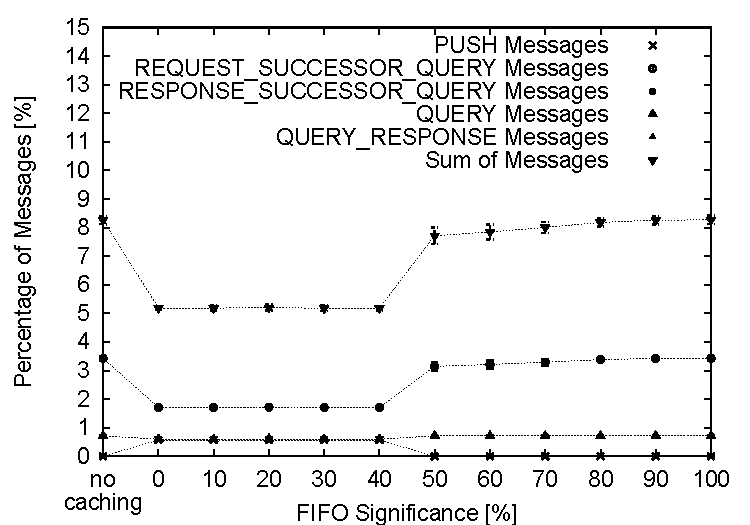
\includegraphics[width=0.48\linewidth]{pic1}}
%  \hspace{0.01\textwidth}
%  %%----start of second subfigure----
%  \subfloat[FIFO size limited to 30 entries]{
%   \label{fig:multipic:b} %% label for second subfigure
%   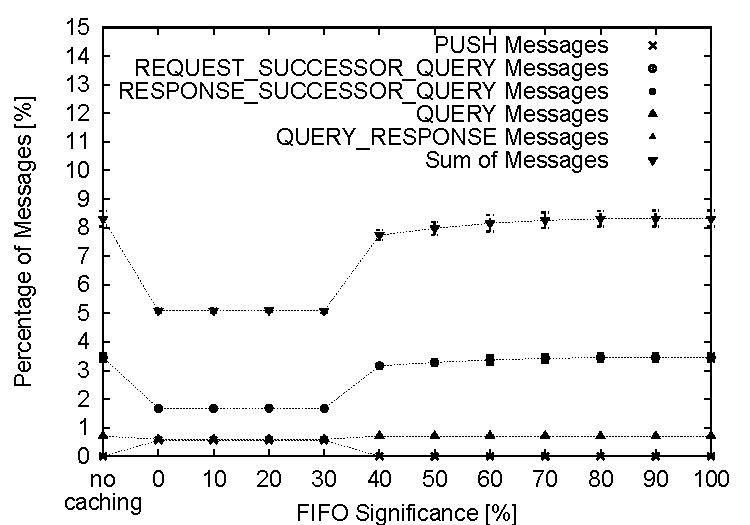
\includegraphics[width=0.48\linewidth]{pic2}}\\[0pt] % horizontal break
%  %%----start of third subfigure----
%  \subfloat[FIFO size limited to 40 entries]{
%   \label{fig:multipic:c} %% label for third subfigure
%   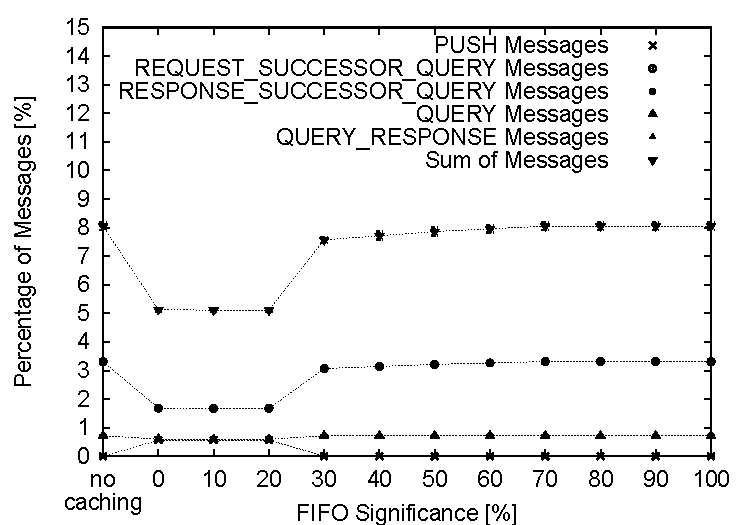
\includegraphics[width=0.48\linewidth]{pic3}}
%  \hspace{0.01\textwidth}
%  %%----start of fourth subfigure----
%  \subfloat[FIFO size limited to 50 entries]{
%   \label{fig:multipic:d} %% label for fourth subfigure
%   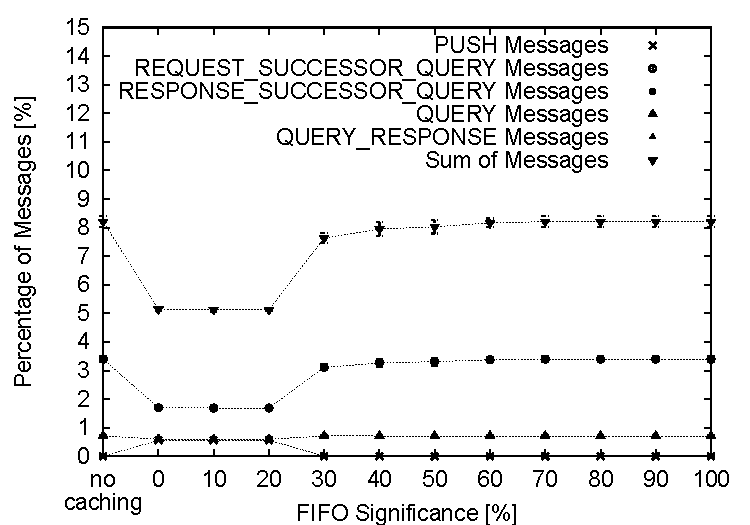
\includegraphics[width=0.48\linewidth]{pic4}}
% \caption[Observed message fractions and 95\% confidence intervals for Chord]{Observed message fractions and 95\% confidence intervals for Chord without the influence of churn. The FIFO capacity varies from 20 (\ref{fig:multipic:a}) -- 50 (\ref{fig:multipic:d}) entries (decadic steps).}
% \label{fig:multipic} %% label for entire figure
%\end{figure}
\section{Interpretation}\label{sec:interpretation}
\subparagraph*{Ergebnisqualität}
\subparagraph*{CPU-Zeit}
\subparagraph*{Speicherbedarf}
\subparagraph*{Komplexität}
\subparagraph*{Aufbaukosten}